% ============================================================
%  Chapter 4 — Local Descent
%  Algorithms for Optimization, 2nd ed. (2026)
%  Kochenderfer & Wheeler
% ============================================================
\documentclass[aspectratio=169,10pt]{beamer}

\usetheme{Madrid}
\usecolortheme{seahorse}

\usepackage{amsmath,amssymb,amsfonts}
\usepackage{mathtools}
\usepackage{booktabs}
\usepackage{listings}
\usepackage{xcolor}
\usepackage{graphicx}
\usepackage{tikz}
\usepackage{array}
\usepackage{hyperref}
\usepackage{microtype}

\graphicspath{{figures/}}

% ── listings style ──────────────────────────────────────────
\lstdefinestyle{pycode}{
  language=Python,
  basicstyle=\ttfamily\scriptsize,
  numbers=left,
  numberstyle=\tiny\color{gray},
  frame=single,
  backgroundcolor=\color{gray!7},
  keywordstyle=\color{blue!70!black}\bfseries,
  commentstyle=\color{green!50!black},
  stringstyle=\color{red!60!black},
  breaklines=true,
  showstringspaces=false,
  tabsize=4,
  xleftmargin=1.5em,
  framexleftmargin=1.5em,
}

% ── convenience macros ──────────────────────────────────────
\newcommand{\bx}{\mathbf{x}}
\newcommand{\bd}{\mathbf{d}}
\newcommand{\bg}{\mathbf{g}}
\newcommand{\bH}{\mathbf{H}}
\newcommand{\bE}{\mathbf{E}}
\newcommand{\R}{\mathbb{R}}
\newcommand{\grad}{\nabla}
\newcommand{\norm}[1]{\left\|#1\right\|}

% ── footer ──────────────────────────────────────────────────
\setbeamertemplate{footline}[frame number]
\setbeamertemplate{navigation symbols}{}

% ── title ────────────────────────────────────────────────────
\title[Ch.4 Local Descent]{Chapter 4: Local Descent}
\subtitle{Algorithms for Optimization, 2nd ed.\ (2026)}
\author{Kochenderfer \& Wheeler}
\institute{MIT Press}
\date{}

% ============================================================
\begin{document}
% ============================================================

\begin{frame}
  \titlepage
\end{frame}

% ── Outline ─────────────────────────────────────────────────
\begin{frame}{Chapter Outline}
  \tableofcontents
\end{frame}

% ============================================================
\section{4.1 Descent Direction Iteration}
% ============================================================

\begin{frame}{Motivation: Multivariate Optimization}
  \begin{columns}[T]
    \begin{column}{0.55\textwidth}
      \textbf{Goal:} minimize $f : \R^n \to \R$
      \begin{itemize}
        \item May be non-convex, may have many local minima
        \item Exact methods (Chapter 3) do not scale to $n \gg 1$
        \item \textbf{Key idea:} iteratively move the design point in a
              direction that \emph{decreases} $f$
      \end{itemize}
      \vspace{0.5em}
      \textbf{Descent direction iteration:}
      \begin{enumerate}
        \item Check local model; if already at a minimum, stop.
        \item Choose a descent direction $\bd^{(k)}$ from the current
              point $\bx^{(k)}$.
        \item Choose a step factor $\alpha^{(k)} > 0$.
        \item Update: $\bx^{(k+1)} \leftarrow \bx^{(k)} + \alpha^{(k)}\bd^{(k)}$.
      \end{enumerate}
    \end{column}
    \begin{column}{0.42\textwidth}
      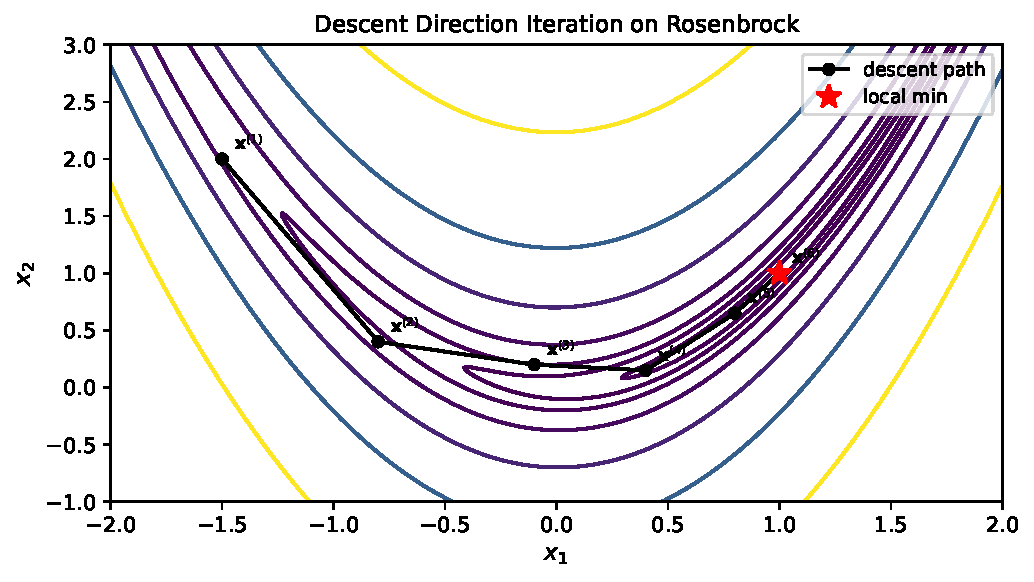
\includegraphics[width=\linewidth]{fig_descent_iteration.pdf}
    \end{column}
  \end{columns}
\end{frame}

\begin{frame}{What Is a Descent Direction?}
  \begin{block}{Definition: Descent Direction}
    A vector $\bd \in \R^n$ is a \emph{descent direction} at $\bx$ if
    \[
      \nabla_{\bd} f(\bx) = \grad f(\bx)^{\top}\bd < 0.
    \]
    The \emph{directional derivative} $\nabla_{\bd}f$ is negative, so
    moving a small positive distance along $\bd$ decreases $f$.
  \end{block}

  \begin{columns}[T]
    \begin{column}{0.48\textwidth}
      \textbf{Properties:}
      \begin{itemize}
        \item The negative gradient $-\grad f(\bx)$ is always a descent
              direction (steepest descent).
        \item Newton direction, quasi-Newton directions are also descent
              directions under suitable conditions.
        \item Momentum directions (e.g.\ in machine learning) can provide
              descent with curvature information.
      \end{itemize}
    \end{column}
    \begin{column}{0.48\textwidth}
      \begin{block}{Iterative Update Rule}
        \[
          \bx^{(k+1)} = \bx^{(k)} + \alpha^{(k)}\bd^{(k)}
        \]
        \vspace{0.3em}
        \begin{tabular}{ll}
          $\bx^{(k)}$    & current design point \\
          $\bd^{(k)}$    & descent direction \\
          $\alpha^{(k)}$ & step factor (step size) \\
        \end{tabular}
      \end{block}
    \end{column}
  \end{columns}
\end{frame}

\begin{frame}[fragile]{Algorithm 4.1: Descent Direction Iteration (Python)}
\begin{lstlisting}[style=pycode]
import numpy as np

def descent_direction_iteration(f, grad_f, x0, direction_fn,
                                 step_fn, max_iter=1000, tol=1e-6):
    """
    Generic descent direction iteration.
    Args:
        f         : objective function  f(x) -> float
        grad_f    : gradient function   grad_f(x) -> ndarray
        x0        : initial design point (ndarray)
        direction_fn: d = direction_fn(x, g) -> descent direction
        step_fn   : alpha = step_fn(f, grad_f, x, d) -> step factor
    """
    x = x0.copy().astype(float)
    history = [x.copy()]
    for k in range(max_iter):
        g = grad_f(x)
        if np.linalg.norm(g) < tol:
            break
        d = direction_fn(x, g)          # choose descent direction
        alpha = step_fn(f, grad_f, x, d) # choose step factor
        x = x + alpha * d
        history.append(x.copy())
    return x, history
\end{lstlisting}
\end{frame}

% ============================================================
\section{4.2 Step Factors}
% ============================================================

\begin{frame}{Step Factors (Learning Rate)}
  \begin{columns}[T]
    \begin{column}{0.55\textwidth}
      The \emph{step factor} (also called \emph{step size} or
      \emph{learning rate}) $\alpha^{(k)}$ controls how far to move.

      \vspace{0.5em}
      \textbf{Fixed step factor:}
      $\alpha^{(k)} = \alpha_0$  for all $k$.
      \begin{itemize}
        \item Simple, but must be chosen carefully.
        \item Too large $\Rightarrow$ divergence.
        \item Too small $\Rightarrow$ slow convergence.
      \end{itemize}

      \vspace{0.4em}
      \textbf{Decaying step factors} allow large early steps (exploration)
      and small later steps (fine-tuning).
    \end{column}
    \begin{column}{0.42\textwidth}
      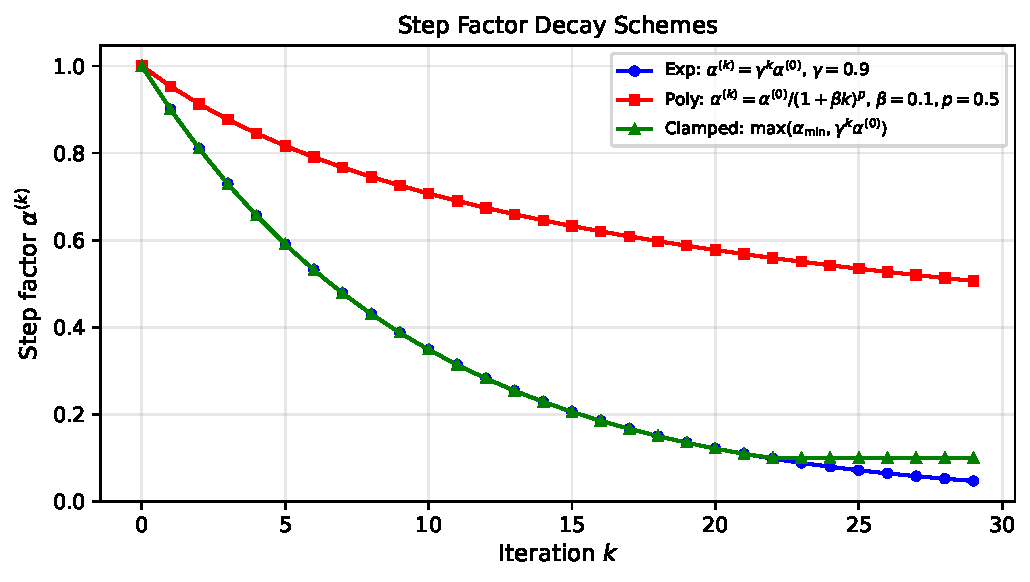
\includegraphics[width=\linewidth]{fig_step_factor_decay.pdf}
    \end{column}
  \end{columns}
\end{frame}

\begin{frame}{Step Factor Decay Schemes}
  \begin{block}{Exponential Decay (Eq.\ 4.2)}
    \[
      \alpha^{(k)} = \gamma^k \alpha^{(0)} = \gamma \alpha^{(k-1)},
      \qquad 0 < \gamma < 1
    \]
    Total distance bounded: $\sum_{k=0}^{\infty} \delta \alpha^{(0)} \gamma^k
    = \dfrac{\delta \alpha^{(0)}}{1-\gamma}$ \quad (if $\|\bd^{(k)}\|\le\delta$)
  \end{block}

  \begin{block}{Polynomial Decay (Eq.\ 4.4)}
    \[
      \alpha^{(k)} = \frac{\alpha^{(0)}}{(1+\beta k)^p}, \qquad \beta>0,\; p>0
    \]
    Unbounded total distance when $0 < p \le 1$.
  \end{block}

  \begin{block}{Clamped Exponential Decay (Eq.\ 4.5)}
    \[
      \alpha^{(k)} = \max\!\left(\alpha_{\min},\, \gamma^k \alpha^{(0)}\right)
    \]
    Prevents premature stagnation; fast early decay, stable later.
  \end{block}
\end{frame}

\begin{frame}[fragile]{Step Factor Decay --- Python Example}
\begin{lstlisting}[style=pycode]
import numpy as np

def exponential_decay(alpha0, gamma, k):
    """alpha^(k) = gamma^k * alpha0,  0 < gamma < 1"""
    return gamma**k * alpha0

def polynomial_decay(alpha0, beta, p, k):
    """alpha^(k) = alpha0 / (1 + beta*k)^p,  beta>0, p>0"""
    return alpha0 / (1.0 + beta * k)**p

def clamped_decay(alpha0, gamma, alpha_min, k):
    """alpha^(k) = max(alpha_min, gamma^k * alpha0)"""
    return max(alpha_min, gamma**k * alpha0)

# Example: gradient descent on f(x) = x^2 with decaying lr
def f(x):   return x**2
def df(x):  return 2*x

x = 3.0
for k in range(20):
    alpha = exponential_decay(alpha0=1.0, gamma=0.85, k=k)
    x = x - alpha * df(x)
    if abs(df(x)) < 1e-6:
        break
print(f"Converged to x={x:.6f}, f(x)={f(x):.2e}")
\end{lstlisting}
\end{frame}

% ============================================================
\section{4.3 Line Search}
% ============================================================

\begin{frame}{Line Search: Optimizing Along a Direction}
  \begin{columns}[T]
    \begin{column}{0.55\textwidth}
      \textbf{Exact line search:} choose $\alpha$ that \emph{minimizes}
      $f$ along the direction $\bd$:
      \[
        \alpha^* = \operatorname*{arg\,min}_{\alpha \ge 0}
                   f\!\left(\bx + \alpha\bd\right)
      \]
      \begin{itemize}
        \item Reduces to 1-D optimization (Chapter 3 methods).
        \item Expensive per iteration if $f$ is costly.
        \item Quadratic $f$: closed-form solution exists.
      \end{itemize}
      \vspace{0.4em}
      \textbf{Quadratic example:}
      For $f(\bx) = \tfrac{1}{2}\bx^{\top}\bH\bx - \bg^{\top}\bx$,
      steepest descent direction $\bd = -\grad f$:
      \[
        \alpha^* = \frac{\bd^{\top}\bd}{\bd^{\top}\bH\bd}
      \]
    \end{column}
    \begin{column}{0.42\textwidth}
      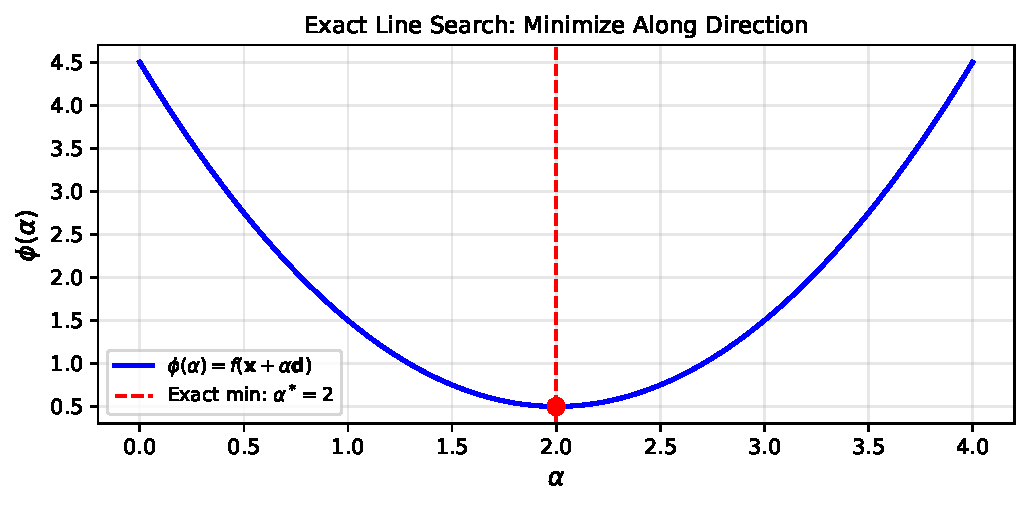
\includegraphics[width=\linewidth]{fig_exact_line_search.pdf}
    \end{column}
  \end{columns}
\end{frame}

\begin{frame}[fragile]{Exact Line Search — Python (SciPy)}
\begin{lstlisting}[style=pycode]
import numpy as np
from scipy.optimize import minimize_scalar

def exact_line_search(f, x, d):
    """
    Minimize f(x + alpha * d) over alpha >= 0.
    Returns optimal step size alpha*.
    """
    phi = lambda alpha: f(x + alpha * d)
    result = minimize_scalar(phi, bounds=(0, 10), method='bounded')
    return result.x

# ── Example: f(x1,x2) = x1^2 + x1*x2 + x2^2 ──────────────
def f(x):
    return x[0]**2 + x[0]*x[1] + x[1]**2

def grad_f(x):
    return np.array([2*x[0] + x[1], x[0] + 2*x[1]])

x = np.array([3.0, 2.0])
d = -grad_f(x)                 # steepest descent direction
alpha_star = exact_line_search(f, x, d)
x_new = x + alpha_star * d

print(f"alpha* = {alpha_star:.4f}")
print(f"x_new  = {x_new}")
print(f"f(x_new) = {f(x_new):.4f}")
\end{lstlisting}
\end{frame}

\begin{frame}{Backtracking Line Search}
  \begin{columns}[T]
    \begin{column}{0.55\textwidth}
      \textbf{Idea:} Start with a large $\alpha$ and reduce it until the
      \emph{sufficient decrease condition} (Armijo, first Wolfe) is met:
      \[
        f(\bx + \alpha\bd) \le f(\bx) + \beta\,\alpha\,\grad f(\bx)^{\top}\bd
      \]
      \begin{itemize}
        \item $\beta \in (0,1)$, typically $10^{-4}$.
        \item Each iteration: $\alpha \leftarrow p\,\alpha$, $p\in(0,1)$,
              typically $p=0.5$.
        \item Guaranteed to terminate if $\bd$ is a descent direction.
        \item Much cheaper than exact line search.
      \end{itemize}
    \end{column}
    \begin{column}{0.42\textwidth}
      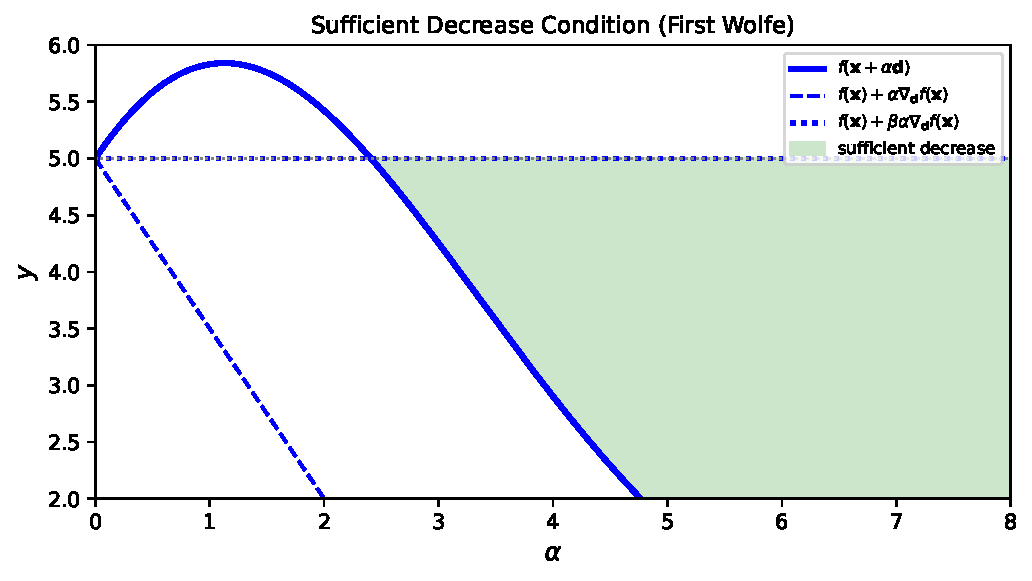
\includegraphics[width=\linewidth]{fig_sufficient_decrease.pdf}
    \end{column}
  \end{columns}
\end{frame}

\begin{frame}{Backtracking on Rosenbrock}
  \begin{columns}[T]
    \begin{column}{0.48\textwidth}
      \textbf{Algorithm 4.3: Backtracking Line Search}
      \begin{enumerate}
        \item $y, \bg \leftarrow f(\bx),\; \grad f(\bx)$
        \item \textbf{while} $f(\bx + \alpha\bd) > y + \beta\alpha(\bg^{\top}\bd)$:
              \begin{itemize}
                \item $\alpha \leftarrow p\,\alpha$
              \end{itemize}
        \item \textbf{return} $\alpha$
      \end{enumerate}
      \vspace{0.5em}
      \textbf{Parameters:}
      \begin{tabular}{ll}
        $\alpha$ & initial step (max step) \\
        $p$      & reduction factor (0.5) \\
        $\beta$  & Armijo parameter ($10^{-4}$) \\
      \end{tabular}
    \end{column}
    \begin{column}{0.48\textwidth}
      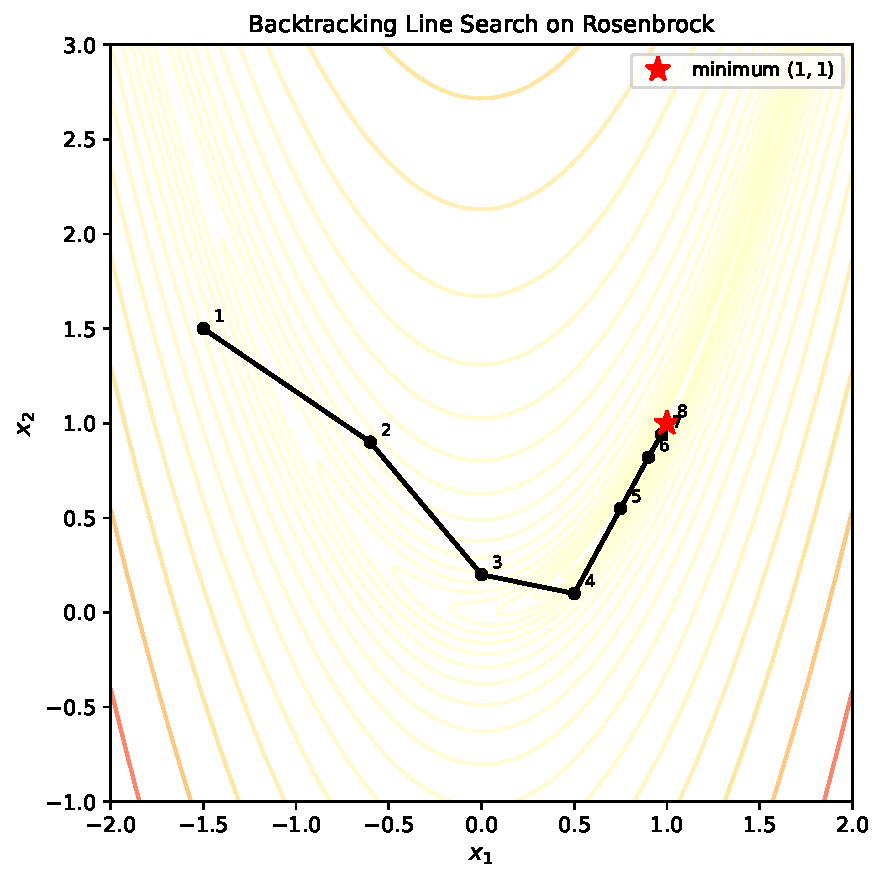
\includegraphics[width=\linewidth]{fig_backtracking_rosenbrock.pdf}
    \end{column}
  \end{columns}
\end{frame}

\begin{frame}[fragile]{Backtracking Line Search — Python}
\begin{lstlisting}[style=pycode]
import numpy as np

def backtracking_line_search(f, grad_f, x, d, alpha=1.0,
                              p=0.5, beta=1e-4):
    """
    Backtracking line search (Armijo condition).
    Reduces alpha by factor p until sufficient decrease is met.
    """
    y = f(x)
    g = grad_f(x)
    slope = g @ d           # directional derivative (must be < 0)
    while f(x + alpha * d) > y + beta * alpha * slope:
        alpha *= p
    return alpha

# ── Numerical example (Example 4.2 from book) ──────────────
# f(x1,x2) = x1^2 + x1*x2 + x2^2, x=[1,2], d=[-1,-1]
def f(x):      return x[0]**2 + x[0]*x[1] + x[1]**2
def grad_f(x): return np.array([2*x[0]+x[1], x[0]+2*x[1]])

x = np.array([1.0, 2.0])   # f(x) = 1 + 2 + 4 = 7
d = np.array([-1.0, -1.0]) # descent direction
g = grad_f(x)               # g = [4, 5]

# Iteration 1: alpha=10  ->  f([1,2]+10[-1,-1]) = f([-9,-8]) = 217 > 6.991
# Iteration 2: alpha=5   ->  f([-4,-3])  = 37   > 6.996
# Iteration 3: alpha=2.5 ->  f([-1.5,-0.5]) = 3.25 <= 6.998  *accept*
alpha = backtracking_line_search(f, grad_f, x, d, alpha=10.0, beta=1e-4)
print(f"Accepted alpha = {alpha}")   # => 2.5
print(f"f(x + alpha*d) = {f(x + alpha*d):.4f}")
\end{lstlisting}
\end{frame}

% ============================================================
\section{4.4 Approximate Line Search — Wolfe Conditions}
% ============================================================

\begin{frame}{Why Approximate Line Search?}
  \begin{itemize}
    \item Exact line search is too costly in practice.
    \item \textbf{Backtracking} only enforces \emph{sufficient decrease} —
          it may accept very small steps.
    \item We want conditions that guarantee the step is:
          \begin{enumerate}
            \item Not too small (\emph{sufficient decrease}).
            \item Not too large (\emph{curvature condition}).
          \end{enumerate}
  \end{itemize}
  \vspace{0.4em}
  \begin{block}{Wolfe Conditions (sufficient decrease + curvature)}
    \textbf{First Wolfe (Armijo):}
    \[
      f(\bx + \alpha\bd) \le f(\bx) + \beta\alpha\,\grad f(\bx)^{\top}\bd
    \]
    \textbf{Second Wolfe (curvature):}
    \[
      \grad f(\bx + \alpha\bd)^{\top}\bd \ge \sigma\,\grad f(\bx)^{\top}\bd
    \]
    with $0 < \beta < \sigma < 1$; typically $\beta=10^{-4}$, $\sigma=0.9$.
  \end{block}
\end{frame}

\begin{frame}{Strong Wolfe Conditions}
  \begin{columns}[T]
    \begin{column}{0.55\textwidth}
      The \emph{strong Wolfe conditions} add an absolute value to the curvature:
      \begin{enumerate}
        \item \textbf{Sufficient decrease:}
              $f(\bx+\alpha\bd) \le f(\bx) + \beta\alpha\,\grad f(\bx)^{\top}\bd$
        \item \textbf{Strong curvature:}
              $\left|\grad f(\bx+\alpha\bd)^{\top}\bd\right| \le
               \sigma\left|\grad f(\bx)^{\top}\bd\right|$
      \end{enumerate}
      \vspace{0.4em}
      \textbf{Why strong?}
      \begin{itemize}
        \item Prevents steps near a local max of $\phi(\alpha)$.
        \item Required by conjugate gradient and quasi-Newton methods.
        \item $\sigma$ close to 1: loose curvature (backtracking-like).
        \item $\sigma$ close to $\beta$: tight, near-exact line search.
      \end{itemize}
    \end{column}
    \begin{column}{0.42\textwidth}
      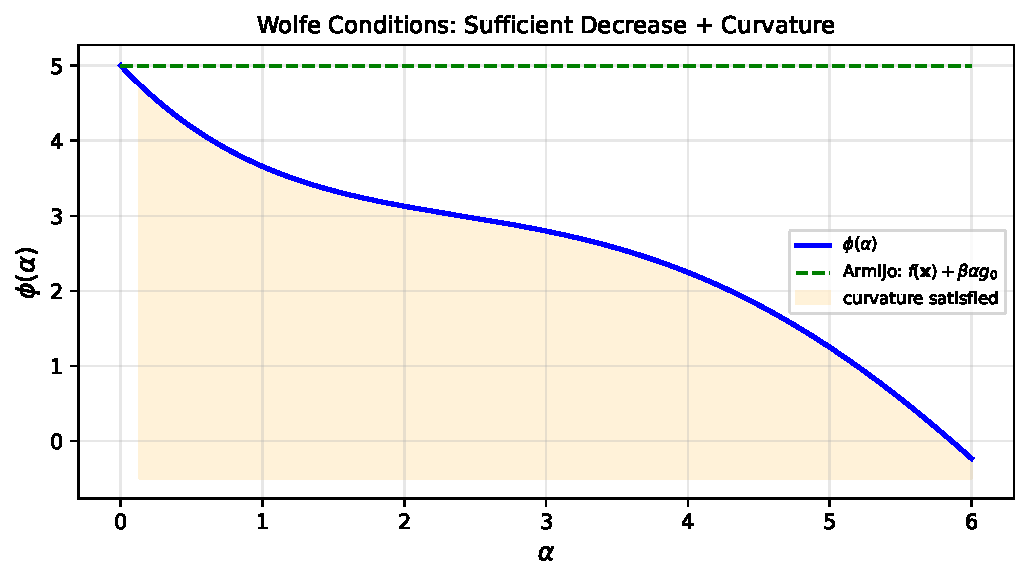
\includegraphics[width=\linewidth]{fig_curvature_condition.pdf}
    \end{column}
  \end{columns}
\end{frame}

\begin{frame}{Strong Backtracking Algorithm}
  \begin{columns}[T]
    \begin{column}{0.52\textwidth}
      \textbf{Algorithm 4.4: Strong Backtracking}

      \textbf{Bracket phase:} Find an interval $[\alpha_{\rm lo},\alpha_{\rm hi}]$
      guaranteed to contain a strong-Wolfe step:
      \begin{itemize}
        \item If $f(\bx+\alpha\bd) > f(\bx) + \beta\alpha g_0$
              or $f(\bx+\alpha\bd) \ge f_{\rm prev}$:
              bracket $[\alpha_{\rm prev}, \alpha]$, go to zoom.
        \item Compute $g = \grad f(\bx+\alpha\bd)^{\top}\bd$.
              If $|g| \le {-\sigma g_0}$: \textbf{return} $\alpha$.
        \item If $g \ge 0$: bracket $[\alpha, \alpha_{\rm prev}]$, zoom.
        \item Else: $\alpha_{\rm prev}\leftarrow\alpha$, $\alpha\leftarrow 2\alpha$.
      \end{itemize}

      \textbf{Zoom phase:} Bisect $[\alpha_{\rm lo},\alpha_{\rm hi}]$ until
      strong Wolfe conditions are satisfied.
    \end{column}
    \begin{column}{0.45\textwidth}
      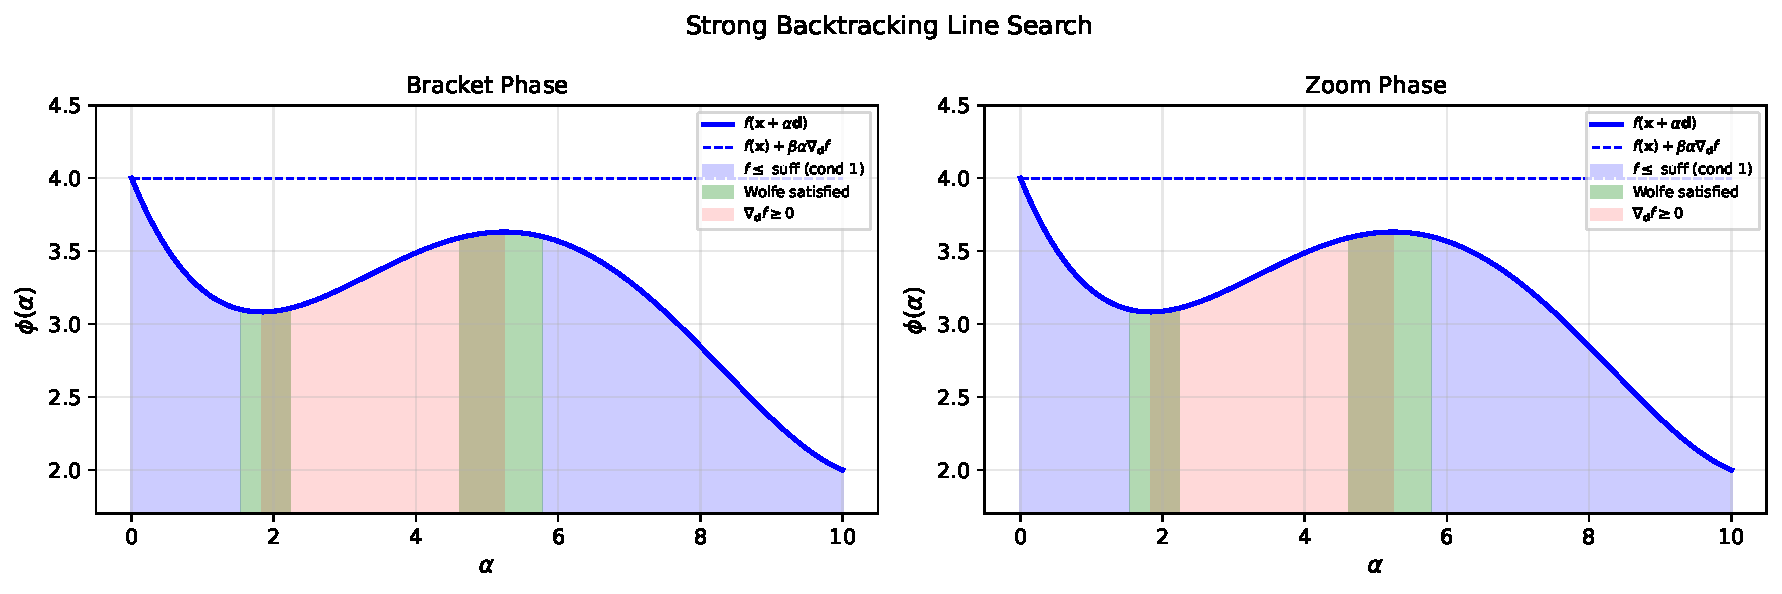
\includegraphics[width=\linewidth]{fig_strong_backtracking.pdf}
      \vspace{0.2em}
      \small
      Left: bracket phase expands $\alpha$ until a bracketing condition
      is triggered. Right: zoom phase bisects the bracket.
    \end{column}
  \end{columns}
\end{frame}

\begin{frame}[fragile]{Strong Backtracking — Python}
\begin{lstlisting}[style=pycode]
import numpy as np

def strong_backtracking(f, grad_f, x, d, alpha=1.0, beta=1e-4, sigma=0.1):
    """Strong backtracking line search satisfying strong Wolfe conditions."""
    y0 = f(x)
    g0 = grad_f(x) @ d          # directional derivative at alpha=0
    y_prev, alpha_prev = float('nan'), 0.0
    alpha_lo = alpha_hi = float('nan')

    # Bracket phase
    while True:
        y = f(x + alpha * d)
        if y > y0 + beta * alpha * g0 or (not np.isnan(y_prev) and y >= y_prev):
            alpha_lo, alpha_hi = alpha_prev, alpha
            break
        g = grad_f(x + alpha * d) @ d
        if abs(g) <= -sigma * g0:
            return alpha                    # strong Wolfe satisfied
        if g >= 0:
            alpha_lo, alpha_hi = alpha, alpha_prev
            break
        y_prev, alpha_prev, alpha = y, alpha, 2 * alpha

    # Zoom phase (bisection)
    y_lo = f(x + alpha_lo * d)
    while True:
        alpha = (alpha_lo + alpha_hi) / 2.0
        y = f(x + alpha * d)
        if y > y0 + beta * alpha * g0 or y >= y_lo:
            alpha_hi = alpha
        else:
            g = grad_f(x + alpha * d) @ d
            if abs(g) <= -sigma * g0:
                return alpha
            if g * (alpha_hi - alpha_lo) >= 0:
                alpha_hi = alpha_lo
            alpha_lo = alpha
\end{lstlisting}
\end{frame}

\begin{frame}{Wolfe Conditions: Bracketing Guarantee}
  \begin{columns}[T]
    \begin{column}{0.55\textwidth}
      An interval $[0, a]$ is \textbf{guaranteed to contain} a step
      satisfying the strong Wolfe conditions when \emph{any} of the
      three bracketing conditions holds:
      \begin{enumerate}
        \item $f(\bx+\alpha\bd) \ge f(\bx)$ \hfill (overshot)
        \item $f(\bx+\alpha\bd) > f(\bx) + \beta\alpha\grad_{\bd}f(\bx)$
              \hfill (violated Armijo)
        \item $\grad_{\bd}f(\bx+\alpha\bd) \ge 0$
              \hfill (gradient changed sign)
      \end{enumerate}
      \vspace{0.5em}
      The zoom phase narrows the interval by bisection, preserving the
      bracket invariant.
    \end{column}
    \begin{column}{0.42\textwidth}
      \begin{block}{Condition Numbers (Eq.\ 4.11--4.13)}
        \[
          f(\bx+\alpha\bd) \ge f(\bx)
        \]
        \[
          f(\bx+\alpha\bd) > f(\bx) + \beta\alpha\nabla_{\bd}f(\bx)
        \]
        \[
          \nabla_{\bd}f(\bx+\alpha\bd) \ge 0
        \]
      \end{block}
    \end{column}
  \end{columns}
\end{frame}

\begin{frame}{Numerical Example: Backtracking (Example 4.2)}
  \begin{block}{Setup}
    $f(x_1, x_2) = x_1^2 + x_1 x_2 + x_2^2$,\quad
    $\bx = [1,2]^{\top}$,\quad
    $\bd = [-1,-1]^{\top}$,\quad
    $\alpha_{\max}=10$,\quad $p=0.5$,\quad $\beta=10^{-4}$.
  \end{block}

  \begin{itemize}
    \item $f(\bx) = 1 + 2 + 4 = 7$,\quad
          $\bg = \grad f(\bx) = [4,5]^{\top}$
  \end{itemize}

  \begin{columns}[T]
    \begin{column}{0.52\textwidth}
      \textbf{Iteration 1:} $\alpha = 10$
      \begin{align*}
        f([1,2] + 10[-1,-1]) &= f([-9,-8]) = 217\\
        7 + 10^{-4}\cdot10\cdot[4,5]^{\top}[-1,-1] &= 6.991\\
        217 \le 6.991 &\;\Rightarrow\; \text{FAIL}
      \end{align*}
      \textbf{Iteration 2:} $\alpha = 5$
      \begin{align*}
        f([-4,-3]) &= 37\\
        37 \le 6.996 &\;\Rightarrow\; \text{FAIL}
      \end{align*}
    \end{column}
    \begin{column}{0.45\textwidth}
      \textbf{Iteration 3:} $\alpha = 2.5$
      \begin{align*}
        f([-1.5,-0.5]) &= 3.25\\
        3.25 \le 6.998 &\;\Rightarrow\; \textbf{ACCEPT}
      \end{align*}
      \vspace{0.5em}
      Final step: $\alpha^* = 2.5$,
      \[
        \bx_{\rm new} = [-1.5, -0.5]
      \]
    \end{column}
  \end{columns}
\end{frame}

% ============================================================
\section{4.5 Trust Region Methods}
% ============================================================

\begin{frame}{Trust Region: Concept}
  \begin{columns}[T]
    \begin{column}{0.55\textwidth}
      \textbf{Idea:} Instead of choosing a \emph{direction} and then a
      \emph{step}, simultaneously choose the step within a trusted region.

      \begin{itemize}
        \item Local quadratic model:
              \[
                \hat{f}(\bx') \approx f(\bx) +
                \grad f(\bx)^{\top}(\bx'-\bx) +
                \tfrac{1}{2}(\bx'-\bx)^{\top}\bH(\bx'-\bx)
              \]
        \item Solve: minimize $\hat{f}$ subject to $\|\bx'-\bx\|\le\delta$
        \item Trust region radius $\delta$ is adapted based on how well
              the model predicts the actual decrease.
      \end{itemize}
    \end{column}
    \begin{column}{0.42\textwidth}
      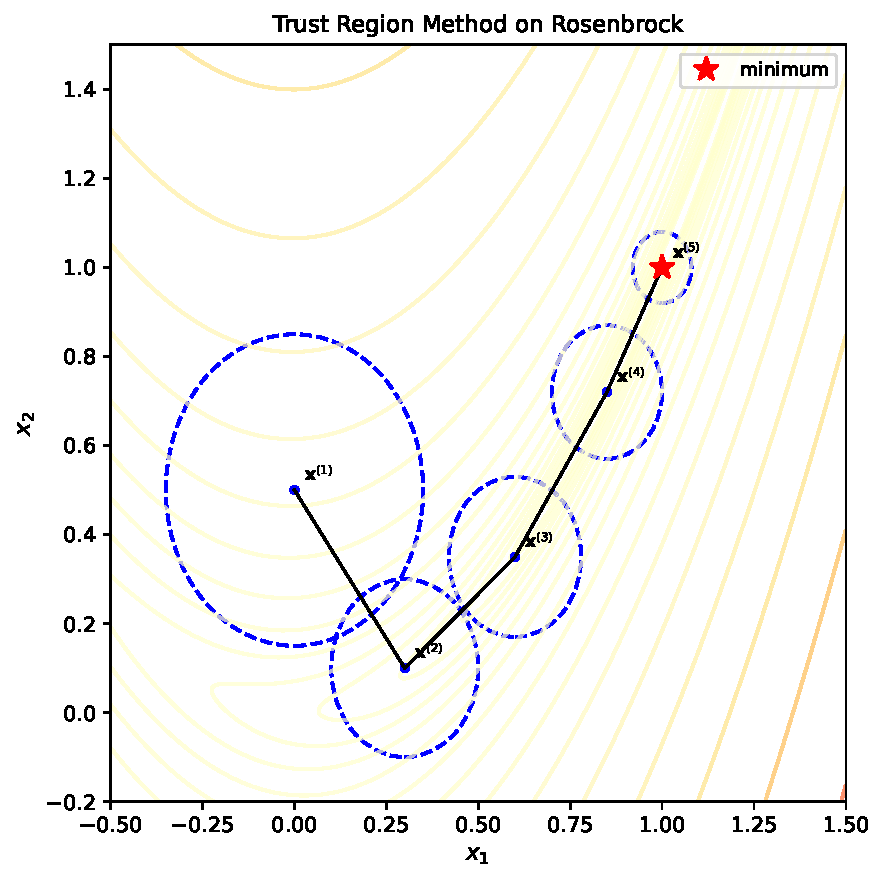
\includegraphics[width=\linewidth]{fig_trust_region.pdf}
    \end{column}
  \end{columns}
\end{frame}

\begin{frame}{Trust Region: Improvement Ratio}
  \begin{columns}[T]
    \begin{column}{0.55\textwidth}
      \begin{block}{Improvement Ratio (Eq.\ 4.15)}
        \[
          \eta = \frac{f(\bx) - f(\bx')}
                      {f(\bx) - \hat{f}(\bx')}
               = \frac{\Delta f_{\rm actual}}
                      {\Delta f_{\rm predicted}}
        \]
        \begin{tabular}{ll}
          $\bx'$ & candidate next point \\
          $\hat{f}(\bx')$ & quadratic model prediction \\
        \end{tabular}
      \end{block}
      \vspace{0.5em}
      \textbf{Trust region update rules:}
      \begin{itemize}
        \item $\eta < \eta_1$ (bad model): shrink $\delta \leftarrow \gamma_1\delta$
        \item $\eta_1 \le \eta \le \eta_2$: keep $\delta$
        \item $\eta > \eta_2$ (good model): expand $\delta \leftarrow \gamma_2\delta$
      \end{itemize}
      Typical: $\eta_1=0.25$, $\eta_2=0.75$, $\gamma_1=0.5$, $\gamma_2=2$.
    \end{column}
    \begin{column}{0.42\textwidth}
      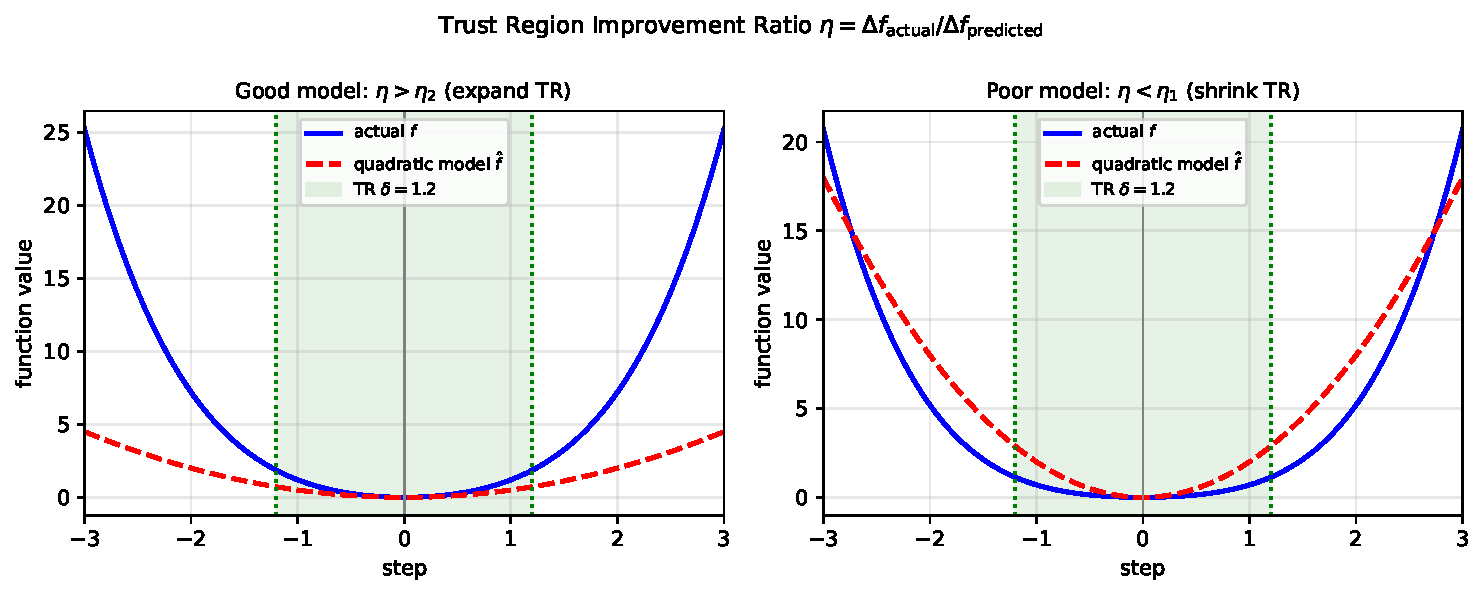
\includegraphics[width=\linewidth]{fig_trust_region_ratio.pdf}
    \end{column}
  \end{columns}
\end{frame}

\begin{frame}{Trust Region Subproblem}
  \begin{block}{Circular Trust Region Subproblem (Eq.\ 4.14)}
    \[
      \bx^{(k+1)} = \operatorname*{arg\,min}_{\bx'}
      \left[ f(\bx^{(k)}) + \grad f(\bx^{(k)})^{\top}(\bx'-\bx^{(k)})
      + \tfrac{1}{2}(\bx'-\bx^{(k)})^{\top}\bH(\bx'-\bx^{(k)}) \right]
    \]
    subject to $\|\bx' - \bx^{(k)}\| \le \delta$
  \end{block}

  \vspace{0.5em}
  \begin{columns}[T]
    \begin{column}{0.48\textwidth}
      \textbf{Elliptical trust region (Eq.\ 4.16):}
      \[
        \|\bx - \bx_0\|_{\bE}^2 = (\bx-\bx_0)^{\top}\bE(\bx-\bx_0) \le 1
      \]
      The matrix $\bE$ elongates the region along directions of
      higher confidence; adapts with each descent step.
    \end{column}
    \begin{column}{0.48\textwidth}
      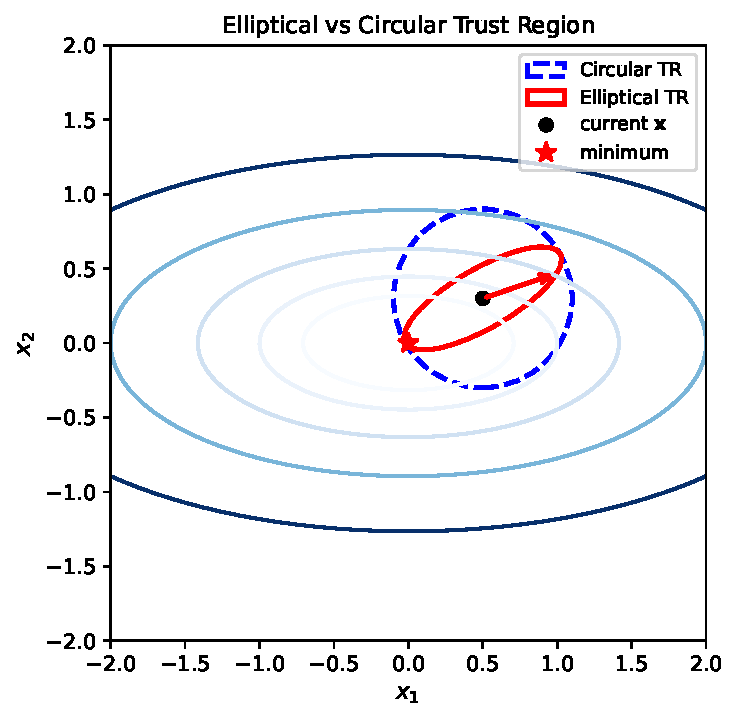
\includegraphics[width=\linewidth]{fig_elliptical_trust_region.pdf}
    \end{column}
  \end{columns}
\end{frame}

\begin{frame}[fragile]{Trust Region Descent — Python (SciPy)}
\begin{lstlisting}[style=pycode]
import numpy as np
from scipy.optimize import minimize

def trust_region_step(grad, hess, x, delta):
    """Solve the trust region subproblem (circular)."""
    n = len(x)
    def model(s):
        return grad @ s + 0.5 * s @ hess @ s
    def model_grad(s):
        return grad + hess @ s
    constraints = {'type': 'ineq',
                   'fun': lambda s: delta - np.linalg.norm(s)}
    s0 = np.zeros(n)
    res = minimize(model, s0, jac=model_grad,
                   constraints=constraints, method='SLSQP')
    return res.x

def trust_region_descent(f, grad_f, hess_f, x0, delta=1.0,
                          eta1=0.25, eta2=0.75,
                          gamma1=0.5, gamma2=2.0, max_iter=100):
    x = x0.copy().astype(float)
    for _ in range(max_iter):
        g = grad_f(x);  H = hess_f(x)
        s = trust_region_step(g, H, x, delta)
        rho = (f(x) - f(x+s)) / (-(g @ s + 0.5 * s @ H @ s))
        if rho > eta1:
            x = x + s          # accept step
        delta = gamma1*delta if rho < eta1 else (gamma2*delta if rho > eta2 else delta)
        if np.linalg.norm(g) < 1e-6: break
    return x
\end{lstlisting}
\end{frame}

% ============================================================
\section{4.6 Termination Conditions}
% ============================================================

\begin{frame}{Termination Conditions}
  \begin{columns}[T]
    \begin{column}{0.55\textwidth}
      When should we stop iterating? Four common criteria:
      \vspace{0.5em}
      \begin{enumerate}
        \item \textbf{Maximum iterations (Eq.\ 4.17):}
              \[ k > k_{\max} \]
        \item \textbf{Absolute improvement (Eq.\ 4.18):}
              \[ f(\bx^{(k)}) - f(\bx^{(k+1)}) < \epsilon_a \]
        \item \textbf{Relative improvement (Eq.\ 4.19):}
              \[ f(\bx^{(k)}) - f(\bx^{(k+1)}) < \epsilon_r \left|f(\bx^{(k)})\right| \]
        \item \textbf{Gradient magnitude (Eq.\ 4.20):}
              \[ \|\grad f(\bx^{(k+1)})\| < \epsilon_g \]
      \end{enumerate}
    \end{column}
    \begin{column}{0.42\textwidth}
      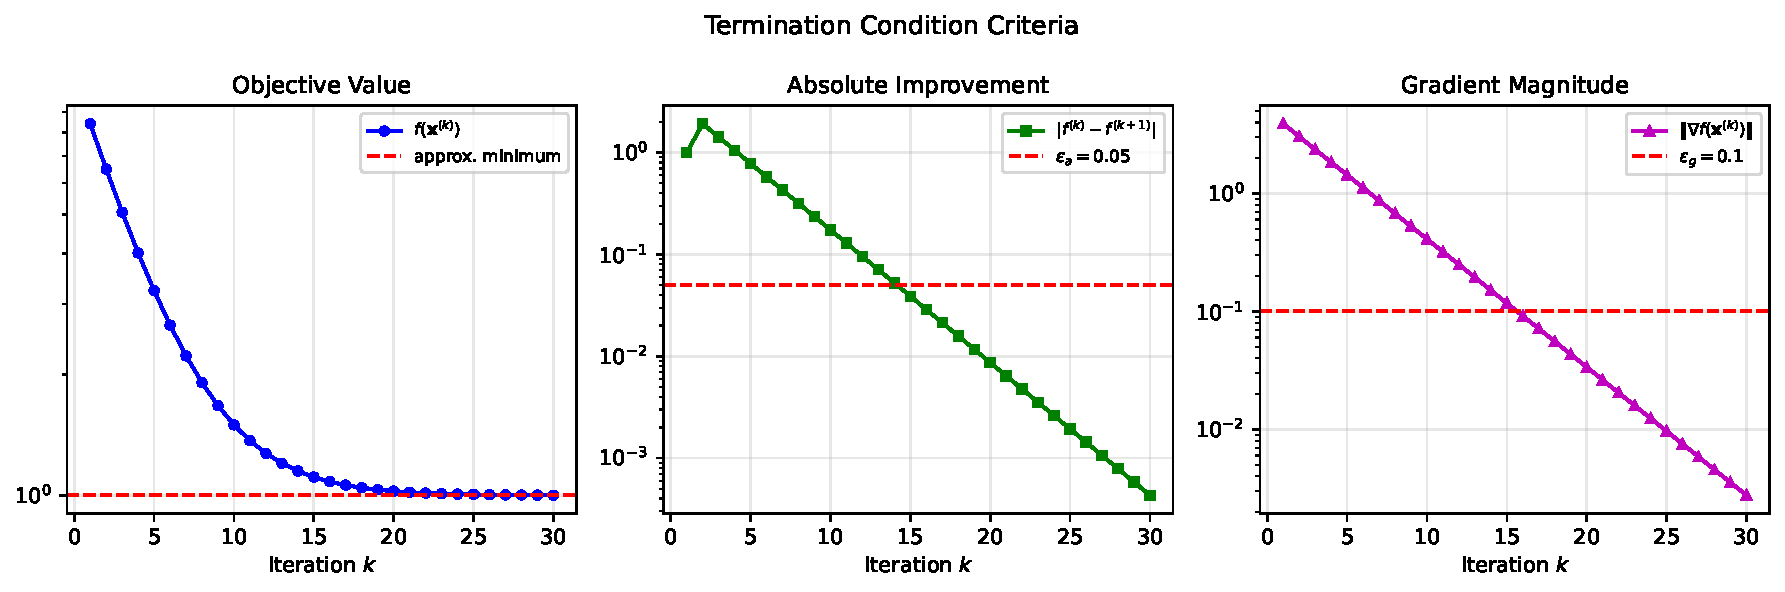
\includegraphics[width=\linewidth]{fig_termination.pdf}
    \end{column}
  \end{columns}
\end{frame}

\begin{frame}{Why Use Multiple Termination Conditions?}
  \begin{columns}[T]
    \begin{column}{0.55\textwidth}
      \textbf{Single condition is fragile:}
      \begin{itemize}
        \item \emph{Max iterations only}: may stop too early or too late.
        \item \emph{Gradient only}: may not converge if $f$ is flat.
        \item \emph{Abs.\ improvement only}: may stall on slow but
              non-zero progress.
      \end{itemize}
      \vspace{0.5em}
      \textbf{Best practice:} combine at least two:
      \begin{itemize}
        \item Gradient + max iterations (safety net).
        \item Add relative improvement for scale-invariance.
      \end{itemize}
      \vspace{0.5em}
      \textbf{Random restarts:} if multiple local minima are likely,
      restart from randomly chosen initial points after each convergence.
    \end{column}
    \begin{column}{0.42\textwidth}
      \begin{block}{Typical Tolerances}
        \centering
        \begin{tabular}{lll}
          \toprule
          Condition & Symbol & Typical value \\
          \midrule
          Max iters     & $k_{\max}$ & $10^3$--$10^5$ \\
          Abs.\ improv. & $\epsilon_a$ & $10^{-8}$ \\
          Rel.\ improv. & $\epsilon_r$ & $10^{-6}$ \\
          Gradient      & $\epsilon_g$ & $10^{-6}$ \\
          \bottomrule
        \end{tabular}
      \end{block}
    \end{column}
  \end{columns}
\end{frame}

\begin{frame}[fragile]{Termination Conditions — Python}
\begin{lstlisting}[style=pycode]
import numpy as np

def check_termination(x_prev, x_curr, f_prev, f_curr, grad_curr,
                       k, k_max=10000, eps_a=1e-8,
                       eps_r=1e-6, eps_g=1e-6):
    """
    Returns (terminated: bool, reason: str).
    Checks all four standard termination conditions.
    """
    if k >= k_max:
        return True, f"max iterations ({k_max})"

    abs_improv = f_prev - f_curr
    if abs_improv < eps_a:
        return True, f"absolute improvement {abs_improv:.2e} < {eps_a}"

    rel_improv = abs_improv / (abs(f_prev) + 1e-12)
    if rel_improv < eps_r:
        return True, f"relative improvement {rel_improv:.2e} < {eps_r}"

    grad_norm = np.linalg.norm(grad_curr)
    if grad_norm < eps_g:
        return True, f"gradient norm {grad_norm:.2e} < {eps_g}"

    return False, "continuing"
\end{lstlisting}
\end{frame}

% ============================================================
\section{4.7 Summary \& Exercises}
% ============================================================

\begin{frame}{Chapter 4 Summary}
  \begin{itemize}
    \item \textbf{Descent direction iteration} provides a general framework:
          choose direction $\bd^{(k)}$ and step $\alpha^{(k)}$,
          update $\bx^{(k+1)} = \bx^{(k)} + \alpha^{(k)}\bd^{(k)}$.

    \item \textbf{Step factors} can be fixed, exponentially decayed,
          polynomially decayed, or chosen by line search.

    \item \textbf{Exact line search} minimizes $f$ exactly along $\bd$
          (costly); \textbf{backtracking} is a cheap alternative.

    \item \textbf{Approximate line search} (Wolfe conditions) balances
          cost and quality:
          \begin{itemize}
            \item First Wolfe (Armijo / sufficient decrease)
            \item Second Wolfe (curvature condition)
            \item Strong Wolfe: $|\grad_{\bd}f(\bx+\alpha\bd)| \le \sigma|\grad_{\bd}f(\bx)|$
          \end{itemize}

    \item \textbf{Trust region methods} replace line search with a
          subproblem constrained to a trust ball of radius $\delta$;
          $\delta$ adapts via the improvement ratio $\eta$.

    \item \textbf{Termination conditions:} use multiple criteria
          (max iterations, absolute/relative improvement, gradient magnitude).
  \end{itemize}
\end{frame}

\begin{frame}{Key Formulas at a Glance}
  \begin{columns}[T]
    \begin{column}{0.48\textwidth}
      \begin{block}{Descent Update}
        $\bx^{(k+1)} = \bx^{(k)} + \alpha^{(k)}\bd^{(k)}$
      \end{block}
      \begin{block}{Step Decay}
        $\alpha^{(k)} = \gamma^k\alpha^{(0)}$
        \quad ($0<\gamma<1$)
      \end{block}
      \begin{block}{First Wolfe (Armijo)}
        $f(\bx+\alpha\bd)\le f(\bx)+\beta\alpha\grad_{\bd}f(\bx)$
      \end{block}
      \begin{block}{Second Wolfe (curvature)}
        $\grad_{\bd}f(\bx+\alpha\bd)\ge\sigma\grad_{\bd}f(\bx)$
      \end{block}
    \end{column}
    \begin{column}{0.48\textwidth}
      \begin{block}{Trust Region Subproblem}
        $\min_{\|\bx'-\bx\|\le\delta}\hat{f}(\bx')$
      \end{block}
      \begin{block}{Improvement Ratio}
        $\eta = \dfrac{f(\bx)-f(\bx')}{f(\bx)-\hat{f}(\bx')}$
      \end{block}
      \begin{block}{Termination}
        $\|\grad f(\bx^{(k+1)})\|<\epsilon_g$\\
        $f(\bx^{(k)})-f(\bx^{(k+1)})<\epsilon_a$
      \end{block}
    \end{column}
  \end{columns}
\end{frame}

\begin{frame}{Exercises}
  \begin{block}{Exercise 4.1}
    Why is it important to have more than one termination condition?
    Give a specific scenario where relying on \emph{only} the gradient
    magnitude condition $\|\grad f\| < \epsilon_g$ would be insufficient.
  \end{block}

  \begin{block}{Exercise 4.2}
    Consider descent applied to $f(x) = \sin(x)$ starting at $x^{(1)}=-2$.
    What is the maximum step size such that $f$ still decreases at each
    iteration (with the negative gradient direction)? Use the first Wolfe
    condition with $\beta=0.1$.
  \end{block}

  \begin{block}{Exercise 4.3 (second-order methods preview)}
    For $f(x_1,x_2)=x_1^2+2x_2^2$, starting at $\bx=[1,1]^{\top}$,
    show that the steepest descent direction is $[-2,-4]^{\top}$ and
    find the exact line search step size $\alpha^*$.
  \end{block}
\end{frame}

\begin{frame}{Further Reading}
  \begin{itemize}
    \item J.\ Nocedal and S.\ J.\ Wright,
          \textit{Numerical Optimization}, 2nd ed.\ Springer, 2006.
          (Convergence analysis of descent methods; trust-region methods.)
    \item A.\ Conn, N.\ Gould, and P.\ Toint,
          \textit{Trust Region Methods}, SIAM, 2000.
          (Definitive reference for trust-region algorithms.)
    \item SciPy documentation: \texttt{scipy.optimize.line\_search\_wolfe2}
          (Strong Wolfe line search),
          \texttt{scipy.optimize.minimize} with \texttt{method='trust-ncg'}.
  \end{itemize}

  \vspace{1em}
  \begin{center}
    \Large\textbf{End of Chapter 4}
  \end{center}
\end{frame}

\end{document}
